\documentclass{article}
\usepackage[utf8]{inputenc}
\usepackage[spanish]{babel}
\usepackage{listings}
\usepackage{graphicx}
\graphicspath{ {images/} }
\usepackage{cite}

\begin{document}

\begin{titlepage}
    \begin{center}
        \vspace*{1cm}
            
        \Huge
        \textbf{Parcial N° 1}
            
        \vspace{2 cm}
        \LARGE
    
            
        \vspace{2 cm}
            
        \textbf{Ivonne  Rosero }\\
        \large
        1007687589
        
        \vspace{2cm}
        \LARGE
        
        \textbf{Rigoberto Berrio}\\
        \large
        1040327583
            
        \vfill
            
        \vspace{0.8cm}
            
        \Large
        Despartamento de Ingeniería Electrónica y Telecomunicaciones\\
        Universidad de Antioquia\\
        Medellín\\
        Abril de 2021
            
    \end{center}
\end{titlepage}

\tableofcontents
\newpage
\section{Análisis del problema y consideraciones para la alternativa de solución propuesta.}\label{intro}
 
Gracias a los apuntes y grabaciones de clase se estan haciendo pruebas para afianzar el conocimiento para poder asimilarlo  al nivel del examen.

Decidimos utilizar 8 integrados para que cada uno controlara 8 leds y asi completar los 64 leds requeridos.

En la Figura (\ref{fig:circuito}) se muestra el circuito a utilizar en el examen.
\begin{figure}[h]
\includegraphics[width=12cm]{circuito.jpg}
\centering
\caption{Circuito final}
\label{fig:circuito}
\end{figure}



\section{Esquema donde describa las tareas que se definieron en el desarrollo del algoritmo.}\label{intro}

1.Buscando reducir al máximo el uso de pines digitales se buscó y a la final lograrlo, puentear 8 integrados 74HC595 en serie; al hacer esto la información dada al primer integrado será la misma que recibirán los demás, esto también nos lleva a conectar los LED’S en grupos de ocho para que cada integrado controle un grupo. Las resistencias tienen la labor de controlar el voltaje ya que los integrados y los leds solo soportan 5V.

2.Se usa el comando shiftOut() la cual se encarga de desplazar hacia la salida un bit cada vez, comienza a partir del bit mas significativo o menos significativo en este caso se inicio desde el bit  menos significativo usando el comando LSBFIRST.
Se programaron los 3 pines que van conectados del arduino al integrado en OUTPUT (salida).
Se obtiene que los leds formen figura.



\newpage
\section{Algoritmo implementado.}\label{intro}
Algoritmo base.
\begin{figure}[h]
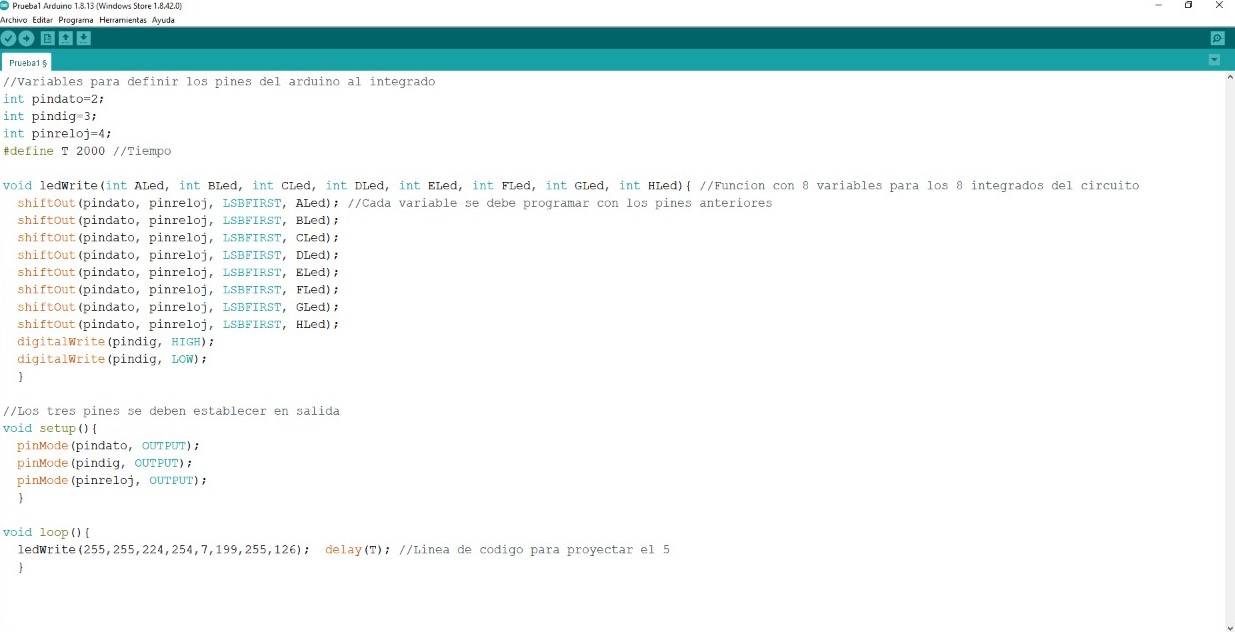
\includegraphics[width=10cm]{Algoritmo.jpeg}
\centering
\caption{Algoritmo Implementado}
\label{fig:Algoritmo}
\end{figure}



\section{Problemas de desarrollo.}\label{intro}
Se usa el comando shiftOut() la cual se encarga de desplazar hacia la salida un bit cada vez, comienza a partir del bit mas significativo o menos significativo en este caso se inicio desde el bit  menos significativo usando el comando LSBFIRST.

Se programaron los 3 pines que van conectados del arduino al integrado en OUTPUT (salida).

Se obtiene que los leds formen la figura.

\begin{figure}[h]
\includegraphics[width=10cm]{figura #5.jpeg}
\centering
\caption{Figura final}
\label{fig:figura #5}
\end{figure}
\newpage
Siempre que el usuario ingrese alguna opcion siempre aparecera de la primero la figura.

Se le muestra al usuario por medio de la funcion "verificacion" que todos los leds funcionan.

\begin{figure}[h]
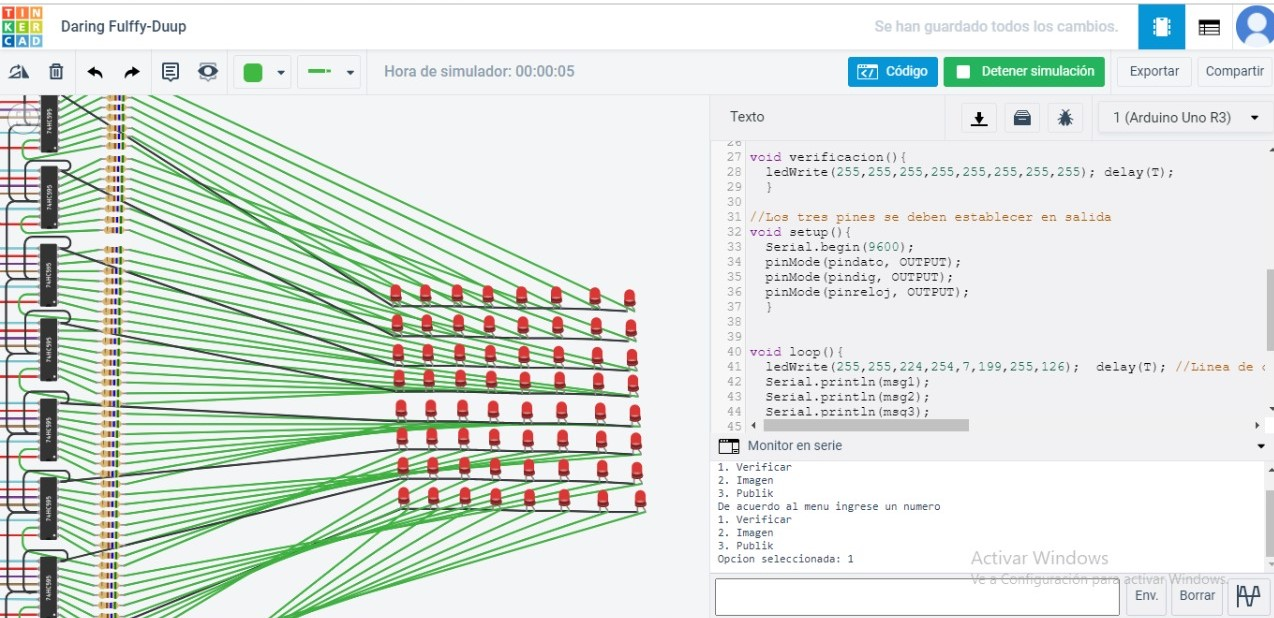
\includegraphics[width=10cm]{Verificacion.jpeg}
\centering
\caption{Verificacion}
\label{fig:Verificacion}
\end{figure}
\newpage

Creacion de la funcion "imagen", en este caso se ingreso que una fila alumbrara y la siguiente no.
\begin{figure}[h]
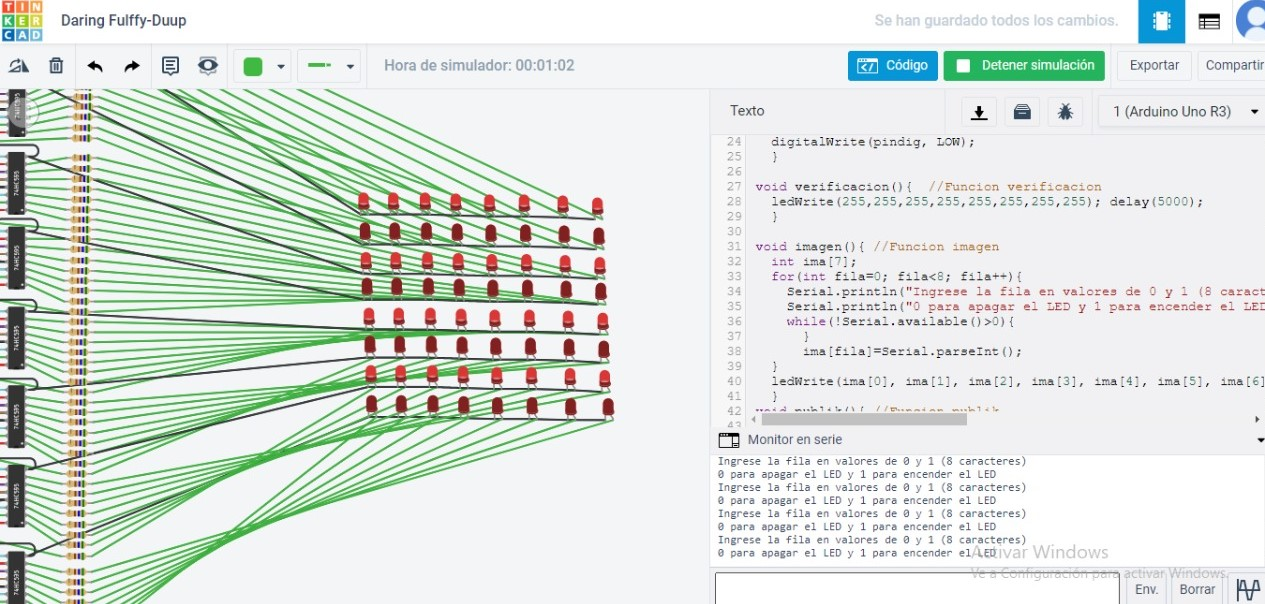
\includegraphics[width=10cm]{Avance 3.jpeg}
\centering
\caption{La imagen que ingreso el usuario.}
\label{fig:Avance 3}
\end{figure}


\section{Evolución del algoritmo y consideraciones a tener en cuenta en la implementación.}\label{intro}
Se crea un menu de manera que el usuario se le facilite la opcion que quiera elegir.

\begin{figure}[h]
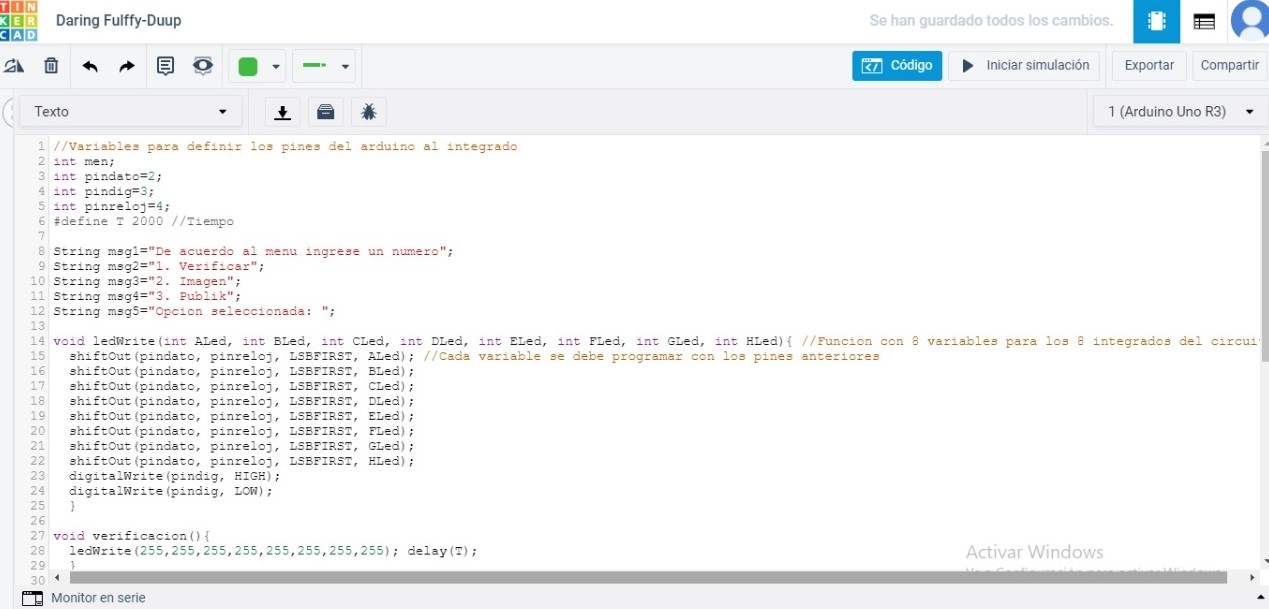
\includegraphics[width=10cm]{Avance 1.jpeg}
\centering
\caption{Avance del codigo}
\label{fig:Avance 1}
\end{figure}
\newpage

En la primera opcion esta la verificación donde el usuario observará que todos los leds funcionan.

\begin{figure}[h]
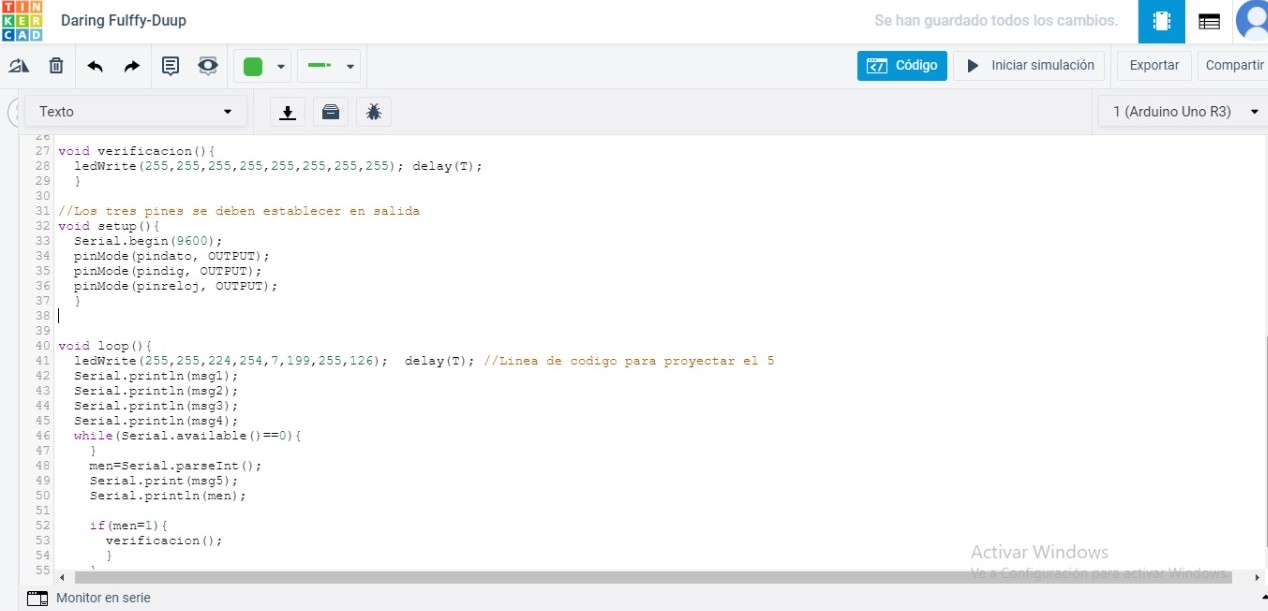
\includegraphics[width=10cm]{Avance 2.jpeg}
\centering
\caption{Avance del codigo}
\label{fig:Avance 2}
\end{figure}


Se crea la funcion "imagen" la cual da la orden a cada led de encender o apagar segun el usuario lo desee ingresando "1" si quiere encenderlo o "0" si desea apagarlo, formando asi la figura que desea.

\begin{figure}[h]
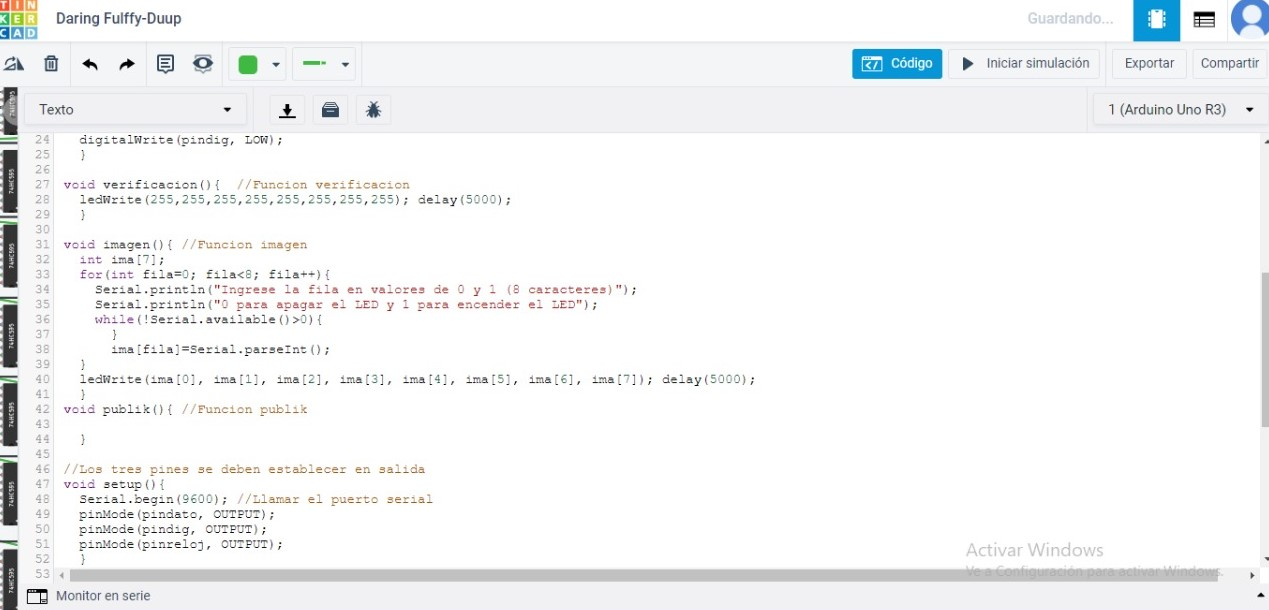
\includegraphics[width=10cm]{Imagen.jpeg}
\centering
\caption{Avance del codigo}
\label{fig:Imagen}
\end{figure}




















\end{document}
